
%(BEGIN_QUESTION)
% Copyright 2010, Tony R. Kuphaldt, released under the Creative Commons Attribution License (v 1.0)
% This means you may do almost anything with this work of mine, so long as you give me proper credit

Et trykkluftsystem har en lekkasje, og du er en del av en gruppe teknikere som har fått i oppdrag å finne lekkasjen. En trykktransmitter som måler trykket i mottakertanken er koblet til en trendregistrator, slik at du kan overvåke tanktrykket over tid. Ved oppsett av lekkasjetesten kjører en tekniker på teamet kompressoren til tankmanometeret viser normalt (fullt) trykk, deretter stopper hun kompressoren og begynner å stenge alle ventilene som er vist (mørke) i denne P\&ID-en:

$$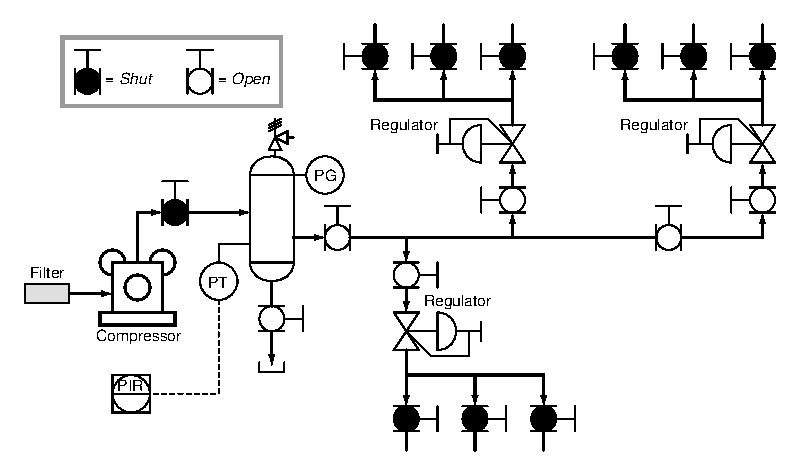
\includegraphics[width=15.5cm]{i01553x01.eps}$$

Etter å ha ventet noen timer undersøker du trenden for mottakertanktrykket, vist her:

$$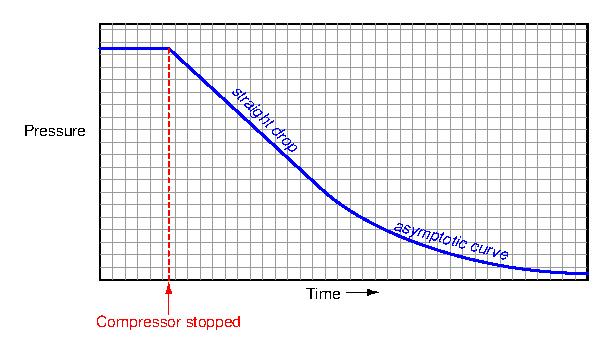
\includegraphics[width=15.5cm]{i01553x02.eps}$$

En annen tekniker på teamet ser denne trenden og utbryter: ``Aha!! Nå vet vi at lekkasjen er nedstrøms en trykkregulator, ikke oppstrøms!'' Forundret ber du kollegaen forklare. ``Se på trendens form: en rett linje med fallende helning, fulgt av en kurve som asymptotisk nærmer seg 0 PSI. Hvis lekkasjen var oppstrøms en regulator, ville hele den fallende trenden vært asymptotisk uten rette deler. Hvis du tar idealgassloven ($PV = nRT$) og uttrykker den som en differensialligning over tid (${dP \over dt} V = {dn \over dt} RT$), ser du at trykkfallets rate ($dP \over dt$) er proporsjonal med lekkasjeraten for luftmolekyler ($dn \over dt$).''

\vskip 10pt

Forklar hva kollegaen din prøver å si, med egne ord. {\it Hvorfor} vil plasseringen av en luftlekkasje i dette systemet gjøre forskjell i {\it formen} på trenden? Videre: hva ville du gjort for å isolere lekkasjens plassering, nå som du vet at den er nedstrøms en regulator?

\vfil 

\underbar{file i01553}
\eject
%(END_QUESTION)





%(BEGIN_ANSWER)

Dette er et vurdert spørsmål -- ingen svar eller hint gitt!

%(END_ANSWER)





%(BEGIN_NOTES)

En lekkasje nedstrøms en trykkregulator vil lekke luft med {\it konstant} rate så lenge det (regulerte) trykket ved lekkasjen er konstant, fordi et konstant trykkfall over en struping er analogt med konstant spenning over en motstand: i begge tilfeller blir resultatet konstant strømning gjennom innsnevringen. Denne konstante luftstrømmen gjennom lekkasjen er det som gjør at mottakertanktrykket faller lineært. Det er samme prinsipp som spenning over en ladet kondensator som lades ut gjennom en strømregulator: spenningsfallets rate mot null ($dU \over dt$) vil være konstant fordi både strømmen ($I$) og kapasitansen ($C$) er konstante størrelser, og de er knyttet sammen med formelen $I = C {dU \over dt}$.

Hvis lekkasjen var oppstrøms en regulator, ville luftlekkasjeraten variert med trykket hele tiden, og gitt et asymptotisk trykkfall hele veien. Med andre ord ville en oppstrøms lekkasje gitt en invers eksponentialkurve som ligner spenningskurven i en motstand-kondensator-utladningskrets.

\vskip 10pt

For å isolere lekkasjen: start kompressoren igjen og bygg opp trykket i mottakertanken, og steng deretter regulatorenes tilførselsventiler én etter én til du ser at trykkfallet flater ut. Trykket skal holde seg stabilt (helning = 0) når det ikke lenger er luftlekkasje.

%INDEX% Mathematics, calculus: differentiation
%INDEX% Measurement, pressure: troubleshooting

%(END_NOTES)

